\subsection{Circuito Rectificador de Onda Completa}

Para éste circuito se usó un transformado con tap central de 12 [V] a 1 [A].\\

\begin{figure}[h!]
    \centering
    \begin{circuitikz}
    
        \draw (0,0) node [transformer](T){};
        \draw  (1,0) to[D,v=$D_1$](3,0); 
        \draw  (1,-2.1) to[D,v=$D_2$](3,-2.1);
        \draw
        (3,0)--(3,-0.9)
        (3,-1.4) arc (-90:90:0.25) 
        (3,-2.1)--(3,-1.4)
        %tap central
        (0.4,-1.15)--(5,-1.15)
        %extension salida
        (3,0)--(5,0)
        %resistor
        (4,0)to[R,l=R](4,-1.15)
        
    
        ; 
    \end{circuitikz}
    \caption{Rectificador Onda Completa}
    \label{fig:rectificadorOndaC}
\end{figure}

En la figura \ref{fig:rectificadorOndaC} se conectó el canal 1 del osciloscopio entre el tap central y el diodo 1, y el canal 2 en el tap central después de las terminales del resistor y en el nodo saliente del diodo 1.\\



\subsection{Circuito de onda completa tipo puente}

\begin{figure}[h!]
    \centering
    \begin{circuitikz}
    
        \draw (0,0) node [transformer](T){};
        \draw  (2,0) to[D,v=$D_1$](4,2); 
        \draw  (4,2) to[D,v=$D_2$](6,0); 
        \draw  (2,0) to[D,v=$D_3$](4,-2);
        \draw  (4,-2) to[D,v=$D_4$](6,0); 
        \draw
        %conexión a D1 y D2
        (1,0)--(1,2)
        (1,2)--(4,2)
        %conexion a D1 y D3
        (2,0)--(2,-3)
        (2,-3)--(3.5,-3)
        (4.5,-3) arc (0:180:0.5)
        (4.5,-3)--(9,-3)
        
        %conexion a D3 y D4
        (1,-2.1)--(1,-4)
        (1,-4)--(4,-4)
        (4,-4)--(4,-2)
        %resistencia extension
        (7,0)to[R,l=$R$](7,-3)
        (6,0)--(9,0)
        ;
       
    \end{circuitikz}
    \caption{Rectificador Onda Completa tipo Puente}
    \label{fig:rectificadorOndaCPuente}
\end{figure}

\begin{figure}
    \centering
    
   
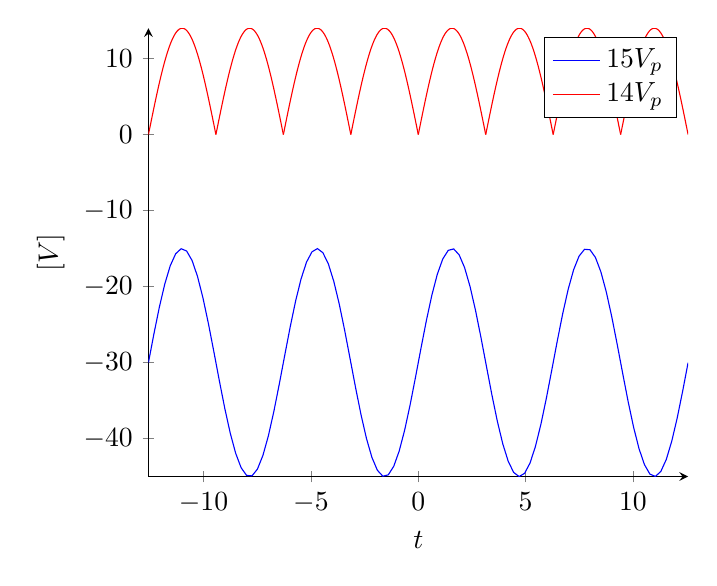
\begin{tikzpicture}
\begin{axis}[
    axis lines = left,
    xlabel = $t$,
    ylabel = {$[V]$},
]


%Entrada al circuito

\addplot [
    domain=-(4*3.14159):+(4*3.14159), 
    samples=100, 
    color=blue,
]
{15*sin(deg(x))-30};

%Onda Rectificada
\addplot [
    domain=-(4*3.14159):+(-3*3.14159), 
    samples=100, 
    color=red,
]
{14*sin(deg(x))};

\addplot [
    domain=-(3*3.14159):+(-2*3.14159), 
    samples=100, 
    color=red,
]
{-14*sin(deg(x))};

\addplot [
    domain=-(2*3.14159):+(-1*3.14159), 
    samples=100, 
    color=red,
]
{14*sin(deg(x))};

\addplot [
    domain=-(1*3.14159):+(-0*3.14159), 
    samples=100, 
    color=red,
]
{-14*sin(deg(x))};

\addplot [
    domain=-(0*3.14159):+(1*3.14159), 
    samples=100, 
    color=red,
]
{14*sin(deg(x))};

\addplot [
    domain=(1*3.14159):+(2*3.14159), 
    samples=100, 
    color=red,
]
{-14*sin(deg(x))};

\addplot [
    domain=(2*3.14159):+(3*3.14159), 
    samples=100, 
    color=red,
]
{14*sin(deg(x))};

\addplot [
    domain=(3*3.14159):+(4*3.14159), 
    samples=100, 
    color=red,
]
{-14*sin(deg(x))};

\addlegendentry{$15 V_{p}$}

    color=blue,
   
 \addlegendentry{$14 V_{p}$}

    color=red,
   
\end{axis}
\end{tikzpicture}

 \caption{Señal circuito rectificador de media onda}
    \label{fig:senalMediaOpuente}
\end{figure}

En la figura \ref{fig:senalMediaOpuente} se puede apreciar el comportamiento de la señal introducida en el circuito de la figura\ref{fig:rectificadorOndaCPuente}\\



\subsection{Circuito rectificador de onda completa bipolar}

\begin{figure}[h!]
    \centering
    \begin{circuitikz}
    
        \draw (0,0) node [transformer](T){};
        \draw  (2,0) to[D,v=$D_1$](4,2); 
        \draw  (4,2) to[D,v=$D_2$](6,0); 
        \draw  (2,0) to[D,v=$D_3$](4,-2);
        \draw  (4,-2) to[D,v=$D_4$](6,0); 
        \draw
        %conexión a D1 y D2
        (1,0)--(1,2)
        (1,2)--(4,2)
        %conexion a D1 y D3
        (2,0)--(2,-3)
        (2,-3)--(3.5,-3)
        (4.5,-3) arc (0:180:0.5)
        (4.5,-3)--(9,-3)
        
        %conexion a D3 y D4
        (1,-2.1)--(1,-4)
        (1,-4)--(4,-4)
        (4,-4)--(4,-2)
        %resistencia extension
        (7,0)to[R,l=$R_1$](7,-1.5)
        (7,-1.5)--(9,-1.5)
        (7,-1.5)to[R,l=$R_2$](7,-3)
        (6,0)--(9,0)
        ;
       
    \end{circuitikz}
    \caption{Rectificador Onda Completa tipo Puente}
    \label{fig:rectificadorOndaCPuenteBipolar}
\end{figure}

en la figura \ref{fig:rectificadorOndaCPuenteBipolar}

\begin{figure}
    \centering
    
   
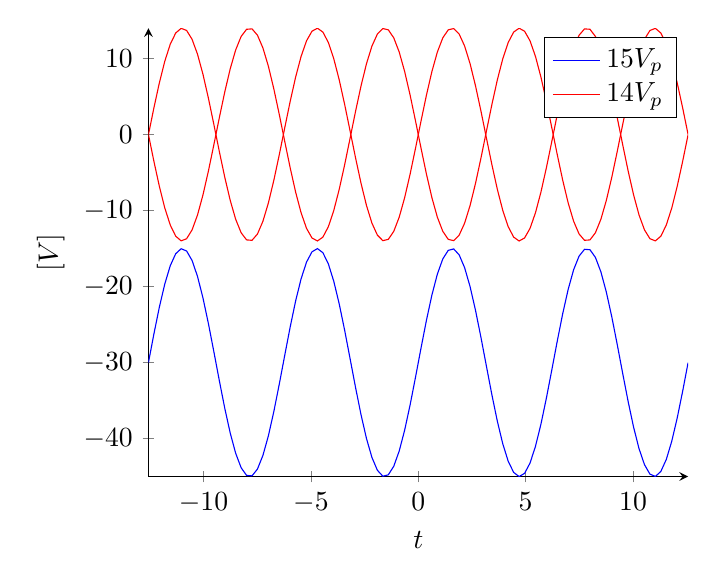
\begin{tikzpicture}
\begin{axis}[
    axis lines = left,
    xlabel = $t$,
    ylabel = {$[V]$},
]


%Entrada al circuito

\addplot [
    domain=-(4*3.14159):+(4*3.14159), 
    samples=100, 
    color=blue,
]
{15*sin(deg(x))-30};

%Onda Rectificada

\addplot [
    domain=-(4*3.14159):+(4*3.14159), 
    samples=100, 
    color=red,
]
{14*sin(deg(x))};
\addplot [
    domain=-(4*3.14159):+(4*3.14159), 
    samples=100, 
    color=red,
]
{-14*sin(deg(x))};



\addlegendentry{$15 V_{p}$}

    color=blue,
   
 \addlegendentry{$14 V_{p}$}

    color=red,
   
\end{axis}
\end{tikzpicture}

 \caption{Señal circuito rectificador de media onda}
    \label{fig:senalMediaOpuentebipolar}
\end{figure}

En la figura \ref{fig:senalMediaOpuentebipolar} se puede apreciar el comportamiento de la señal introducida en el circuito de la figura\ref{fig:rectificadorOndaCPuenteBipolar}, para éste experimento se usaron los dos canales del osciloscopio, en las terminales de los dos resistores, para poder observar el espectro completo del voltaje bipolar de la fuente.\\


\subsection{Rectificador de onda completa}

Un rectificador de onda completa es un circuito empleado para convertir una señal de corriente alterna de entrada (Vi) en corriente de salida (Vo) pulsante. A diferencia del rectificador de media onda, en este caso, la parte negativa de la señal se convierte en positiva o bien la parte positiva de la señal se convertirá en negativa, según se necesite una señal positiva o negativa de corriente continua.

Existen dos alternativas, bien empleando dos diodos o empleando cuatro (puente de Graetz).\citep{circuitoOnda}